\documentclass[10pt]{IOS-Book-Article}
%%%%%%%%%%%%%%%%%%%%%%%Marc version
\usepackage{mathptmx}
\usepackage{graphicx}
\usepackage{subfigure}
\usepackage{fancyvrb}
\usepackage{caption}
%\usepackage{times}
%\normalfont
%\usepackage[T1]{fontenc}
%\usepackage[mtplusscr,mtbold]{mathtime}

%\usepackage{setspace}
%\setstretch{2}

%\mag 2500

\begin{document}
\begin{frontmatter}              % The preamble begins here.

%\pretitle{Pretitle}
\title{Divide and Conquer Parallelization of Finite Element Methods Assembly}
\runningtitle{D\&C Assembly}
%\subtitle{Subtitle}

\author[A]{\fnms{Lo\"ic} \snm{Th\'ebault}%
\thanks{Corresponding Author E-mail: loic.thebault@prism.uvsq.fr}},
\author[A]{\fnms{Eric} \snm{Petit}},
\author[C]{\fnms{Marc} \snm{Tchiboukdjian}},
\author[B]{\fnms{Quang} \snm{Dinh}},
and
\author[A,C]{\fnms{William} \snm{Jalby}}

\runningauthor{L. Th\'ebault et al.}
\address[A]{PRISM - University of Versailles, France}
\address[B]{Dassault Aviation, Saint-Cloud, France}
\address[C]{Exascale Computing Research, France}

\begin{abstract}
Relying solely on domain decomposition and distributed memory parallelism can limit the performance on current supercomputers.
At scale, a larger number of smaller domains can lead to an increased communication volume and to load balancing issues.
Moreover, the decreasing memory per core is not compatible with the memory overhead of a finer domain decomposition.
A popular alternative is to use shared memory parallelism in addition to the domain decomposition.
In the context of Finite Element Methods, FEM, one of the challenging steps to parallelize in shared memory is the matrix assembly.
In this paper, we propose and evaluate a Divide and Conquer, D\&C, algorithm to efficiently parallelize the FEM assembly.
We compare this hybrid approach using D\&C to the pure domain decomposition and to a state-of-the-art hybrid approach using mesh coloring.
Our target application is an industrial fluid dynamics code, developed by Dassault Aviation, parallelized with MPI domain decomposition.
The original Fortran code has been modified with minimum intrusion. Our D\&C approach uses task parallelism with Intel Cilk+.
Preliminary results show good data locality and a 14\% performance improvement on a 12 cores 2 sockets Westmere-EP node.
\end{abstract}

\begin{keyword}
Divide and Conquer, Task, Cilk, Mesh Partitioning, CFD, FEM Assembly
\end{keyword}
\end{frontmatter}

\thispagestyle{empty}
\pagestyle{empty}

\section{Introduction}
\label{sec:intro}
%Current algorithms and runtimes struggle to scale to a large number of cores and show a poor parallel efficiency.
%The increasing number of cores and parallel units implies a lower memory per core, higher requirement for concurrency, higher coherency traffic and higher cost for coherency protocol.
%It results in a severe challenge for performance scalability.
%The manycore accelerators, such as the Intel Xeon Phi, exacerbate these issues. HPC users have to explore new paradigms.

%In order to mitigate the node scalability issues, users can modify their application using hybrid MPI + threads to take advantage of the full topology of the machine
%and enhance the data and synchronization locality.
%In this paper, we propose and evaluate a new parallelization strategy based on the Divide and Conquer, D\&C, principle on unstructured problem.
%Our implementation relies on a task based runtime, Cilk~\cite{cilk5}. 

Relying solely on domain decomposition and distributed memory parallelism can limit the performance on current supercomputers.
At scale, a larger number of smaller domains can lead to an increased communication volume and to load balancing issues.
Moreover, the decrease of the memory per core is not compatible with the memory overhead of a finer domain decomposition.
A popular alternative is to use shared memory parallelism in addition to the domain decomposition.

In the context of Finite Element Methods, FEM, one of the challenging steps to parallelize in shared memory is the matrix assembly.
This step builds from the mesh a sparse matrix describing the linear system of equations.
A simple FEM assembly illustration of a 2D regular mesh is presented in Figure~\ref{fig:2Dasm} with the associated sparse matrix.
The non-zero values of the matrix correspond to the edges of the mesh. These values are the reduction of neighboring elements contribution.
 In Figure~\ref{fig:2Dasm}, $(N1,N2) = E1 + E2$. This matrix is sparse and symmetrical, thus we only need to store the non-zero values in the lower triangle. In 3D, even with a fix number of edges per element, the number of neighboring elements can be arbitrarily large.
Due to the irregularity of the structure and the serialization of the reduction, the FEM assembly cannot be parallelized using a simple parallel loop.


\begin{figure}[htp]
 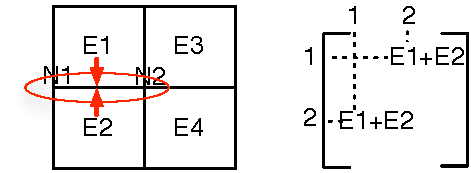
\includegraphics[scale=0.6]{FEM_ass.pdf}
 \caption{A 2D FEM assembly example. The matrix non-zero values correspond to the edges of the mesh.}
 \label{fig:2Dasm}
\end{figure}


The easiest solution to handle the reductions on mesh edges is to use atomic operations.
However, as the amount of computation per edge is usually low, this approach is inefficient.
The state-of-the-art approach for shared memory parallelization is mesh coloring, but it results in a bad data locality as shown in Section~\ref{sec:col}.
Recent works published on parallelizing FEM assembly codes are designed for GPUs~\cite{cecka2011assembly,CPUGPUasm} and can not be efficiently applied to multicore architectures.

In this paper, we propose a new approach based on Divide and Conquer, D\&C, to parallelize the FEM assembly step.
We evaluate this algorithm on an industrial Computational Fluid Dynamics, CFD, code from Dassault Aviation.
This code computes the effect of mesh deformation to optimize airplane structure.
The D\&C approach outperforms the original implementation based on domain decomposition and the coloring method.

The paper is structured as follows.
\begin{itemize}
\item Section~\ref{sec:assembly} presents  two algorithms for the FEM assembly step parallelization: the mesh coloring approach and our D\&C proposal.
\item Section~\ref{sec:exp} presents the experimental evaluation on the DEFMESH application from Dassault Aviation.
\item Section~\ref{sec:rw} and~\ref{sec:conc} presents the related work and the conclusion.
\end{itemize}

%---------------------------------------------------------------------------
%---------------------------------------------------------------------------
%---------------------------------------------------------------------------
%---------------------------------------------------------------------------

\section{FEM Assembly Parallelization Using Shared Memory}
\label{sec:assembly}
Matrix assembly is common in most scientific applications using finite element methods. 
To extract the parallelism from the FEM assembly, we must build independent domains to be executed in parallel. We then synchronize them to handle shared edges.
We consider two different approaches, a state-of-the-art coloring approach and our proposed D\&C strategy based on a topological recursive bisection.


\subsection{Mesh Coloring}
\label{sec:col}
Mesh coloring avoids race conditions by assigning a different color to the elements sharing an edge.
It originally targeted vector machines, indeed elements of a same color do not contribute to the same edges and thus can be executed in parallel.
Determining a minimal coloring is NP-complete, but creating an efficient coloring with a larger number of colors using heuristic is well-known in literature~\cite{CPUfe}.
A pseudo-code and a simple 2D coloring example are given in Figure~\ref{fig:colApp}.

%Despite mesh coloring is an efficient approach for vector machines, it is not well suited for current shared memory parallel architectures.
Sorting the elements by color improves the spatial locality and enables vectorization.
However, each color covers the whole domain and accesses every edges only once.
For large domains, there will be no edge locality in cache between colors.

\begin{SaveVerbatim}[]{VerbCol}
NodeToElem = build_node_element (ElemToNode)
ElemToElem = build_element_element (NodeToElem)
ElemToColor = build_element_color (ElemToElem)
ColorToElem = build_color_element (ElemToColor)

For each color C in colors
  Parallel_For all elements E in C
    compute_element_contribution (E)
\end{SaveVerbatim}

\begin{figure}[htp]
\subfigure[\label{fig:example_coloring}Example of a 2D coloring.]{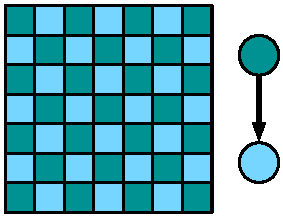
\includegraphics[width=0.3\textwidth]{color.pdf}}
\subfigure[\label{fig:algo_coloring}Pseudo code for coloring and assembling.]{\BUseVerbatim[fontshape=it,fontsize=\footnotesize,fontfamily=courier]{VerbCol}}
\caption{The state-of-the-art coloring approach for FEM assembly.}
\label{fig:colApp}
\end{figure}

\subsection{Divide and Conquer}
\label{sec:dc}
%The D\&C approach is particularly interesting for its ability to scale naturally to an increasing number of node thanks to its architecture oblivious concept.
%Each leaves is responsible of its own data and there is a very minimal amount of sharing, avoiding costly locks and coherency protocols. 

The main idea of our D\&C approach for shared memory parallelization is to enable task level parallelism while preserving good data locality and minimizing synchronization cost.
When the size of the domain increases, we increase the number of tasks and threads instead of increasing the number of MPI domains and the amount of communication.
This way, we take benefit of replacing communication by data sharing.

The rational is to recursively divide the work in two or more independent tasks and synchronize these tasks locally.
This recursive approach has many advantages.
First the recursive sharing naturally exposes high concurrency.
As long as the data-set is large enough, it is possible to produce a deeper recursive tree to get more concurrency and therefore match the higher requirement of manycore systems.
Furthermore, unlike in the coloring approach, no global barrier is needed.
Synchronizations are local: only nodes of a same parent in the recursive tree have to be synchronized.
Finally, D\&C approach improves the data locality by reordering the data as shown in Section~\ref{sec:DCrec}.

In the D\&C approach, the code will benefit from the higher locality and reuse of elements.
Therefore all the versions using the reordering should outperform the original code.

With a small number of cores, the scalability of the D\&C parallelization is expected to be equivalent to the MPI domain decomposition, since we add no significant work to the sequential path.
Furthermore, contrary to the MPI approach, the D\&C algorithm complexity is independent from the number of cores and should continue scaling.


D\&C consists of two parts described in following subsections.
The first part is the recursive decomposition of each MPI domain and the second is the recursive execution of the FEM assembly step using Cilk.

\subsubsection{Recursive Bisection}
\label{sec:DCrec}
D\&C is based on topological recursive bisections of the mesh.
As illustrated in Figure~\ref{fig:DCapp}, the left and right sub-domains created by these bisections do not share any element and can be executed in parallel.
However, the separator elements in the middle have nodes on both sides and must be processed after the left and right sub-domains.
The load balancing between the sub-domains is important since it influences the depth of the recursive tree.
A balanced tree will minimize the maximum depth and thus the number of synchronization on the critical path.
Therefore, it is important to use a good partitioner to build equal sub-domains.
In this study, we use the METIS graph partitioner~\cite{Metis}.

In order to increase the data locality, we permute the nodes and the elements arrays.
As a result, the nodes and the elements can be consecutive in memory inside each sub-domain, improving intra-task locality.
Secondly, since the tasks distribution is following the recursive domain decomposition, we store neighboring sub-domains and their associated separator contiguously to improve locality between tasks.
These permutations are applied to all MPI domains, therefore we renumber the nodes on the frontier so that exchanged data are consistent.
The proposed approach is then applied recursively to all sub-domains, providing a large amount of parallelism.
As illustrated in Figure~\ref{fig:DCrec}, each leaf of the resulting tree is associated with an independent Cilk task which executes the FEM assembly process on its sub-domain.

The partitioning is topological, cuts are done on edges rather than on geometrical coordinates.
This allows to only compute sub-domains once for a mesh and it is independent from the rest of the computation.
Therefore, the partitioning is precomputed and the associated permutation is stored with the mesh.
During the run, the application needs to apply the precomputed permutation before executing the recursive FEM assembly.

\begin{SaveVerbatim}[]{VerbDC}
function compute (subdomain) 
  if Node is not a leaf
    spawn compute (subdomain.left)
    compute (subdomain.right)
    synchronize
    compute (subdomain.sep)
  else
    FEM_assembly (subdomain)
end    
\end{SaveVerbatim}

\begin{figure}[htp]
\subfigure[\label{fig:DCapp}]{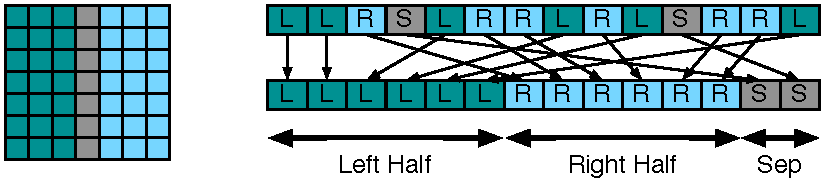
\includegraphics[width=0.7\textwidth]{dc_app.pdf}}
\subfigure[\label{fig:DCrec}]{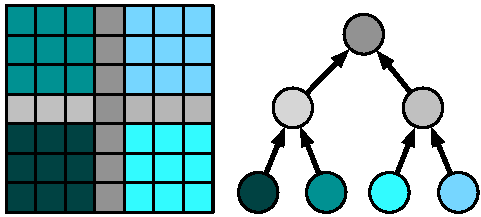
\includegraphics[width=0.49\textwidth]{dc_rec.pdf}}
\subfigure[\label{fig:DCpc}]{\BUseVerbatim[fontshape=it,fontsize=\footnotesize,fontfamily=courier]{VerbDC}}
\caption{D\&C recursive execution. The left and right parts can be treated in parallel.
The edges on the cut form a separator treated after these left and right parts.
For each cut, we reorder the elements in left, right and separator parts.}
\end{figure}

\subsubsection{Cilk Implementation}
Cilk~\cite{cilk5} is a task based runtime originally developed by Frigo, Leiserson and Randal at MIT and now supported by Intel.
It allows users to {\tt spawn} and {\tt sync} efficiently many parallel tasks.
All these tasks are organized in queues and executed by \emph{worker} threads.
For load balancing, Cilk runtime uses a work-stealing scheduler.
When a \emph{worker} completes its queue, it can steal additional tasks from slower \emph{workers}.

Once the recursive task tree, as shown in Figure~\ref{fig:DCrec}, is constructed, the Cilk implementation is straightforward.
Following the pseudo-code in Figure~\ref{fig:DCpc}, left and right sub-domains of each node are split in two tasks and executed in parallel, as long as the recursion has not reached a leaf (domain size condition).
When the recursion reaches the leaves, the original sequential FEM assembly routine is executed on each leaf sub-domain.
The left and right tasks have to be completed before launching the separator computation. 


When all elements are accessed in a regular loop, there is no need to use a recursive task tree.
In this case, similarly to OpenMP, Cilk provides an easy way to parallelize loops using the { \tt cilk\_for} keyword.
By substituting the original {\tt for} with the {\tt cilk\_for} keyword, iterations of the loop are split recursively in several parallel tasks.
For the DEFMESH application, we observe a better scalability with the {\tt cilk\_for} than with OpenMP {\tt parallel for} pragma.

%---------------------------------------------------------------------------
%---------------------------------------------------------------------------
%---------------------------------------------------------------------------
%---------------------------------------------------------------------------

\section{Experiments}
\label{sec:exp}
To validate our approach, we apply the D\&C algorithm using Cilk and MPI on the FEM assembly step of the DEFMESH application developed by Dassault Aviation.
We compare our results with the original MPI domain decomposition version of the FEM assembly step and with the hybrid MPI + OpenMP version using the coloring approach.

\subsection{Dassault Aviation DEFMESH Application}
The DEFMESH application is a CFD code based on FEM.
This volume mesh deformer is an important numerical module in Dassault Aviation aerodynamic optimization environment.
It is also used in other simulations which may include surface variations of larger magnitude, such as in aero-elastic interactions or dynamics of moving bodies.

DEFMESH implements a three-dimensional elasticity-like system of equations from given surface data.
These equations are solved by two different algorithms.
The first one is a linear algorithm used when the magnitude of the surface data is small: the equations can be linearized into a system of linear equations.
The second one is a non-linear algorithm where surface data of large magnitude are cut in a succession of small increments.
The original equations are solved as a non-linear succession of linearized sub-problems, consisting of systems of linear equations.
Each linear system is described as a symmetric definite positive matrix.
The systems are solved by a standard conjugate gradient, CG, algorithm.

DEFMESH implements two options for the definition of the operator for its system of volume equations.
The first one is the Laplacian operator. It calls three times the CG algorithm at each linearized step.
Each CG call computes the solution of a scalar system of linear equations.
The second one is the Elasticity operator. This option implements the full 3D linear Elasticity operator.
It couples the three mesh coordinates, thus at each linearized step, the CG algorithm has to solve a 3 by 3 system of linear equations.
The Elasticity operator permits mesh deformations of greater magnitude and smoother deformed meshes than the Laplacian operator.

The DEFMESH main kernel is decomposed in three steps.
The first one is the FEM assembly, where mesh data are gathered into a sparse matrix.
The second step is the solver which works on this matrix and computes optimal displacements.
The final step is the update of mesh coordinates using previously computed deformations.

We performed our experiments on an unstructured mesh from Dassault Aviation called EIB and illustrated in the Figure~\ref{fig:reservoir}.
It is composed of 6~346~108 elements and 1~079~758 nodes and it represents the displacements of a fuel tank along an airplane fuselage.

\begin{figure}[htp]
 \subfigure[]{\label{fig:EIB3D}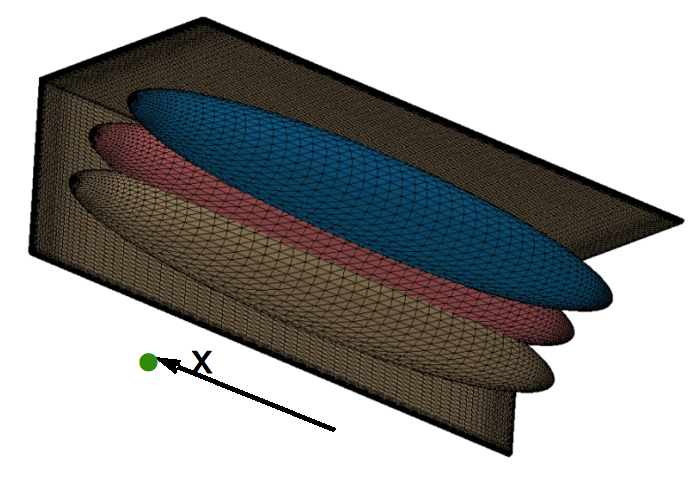
\includegraphics[width=0.28\textwidth]{reservoir_3D.png}}
 \subfigure[]{\label{fig:EIB_proj}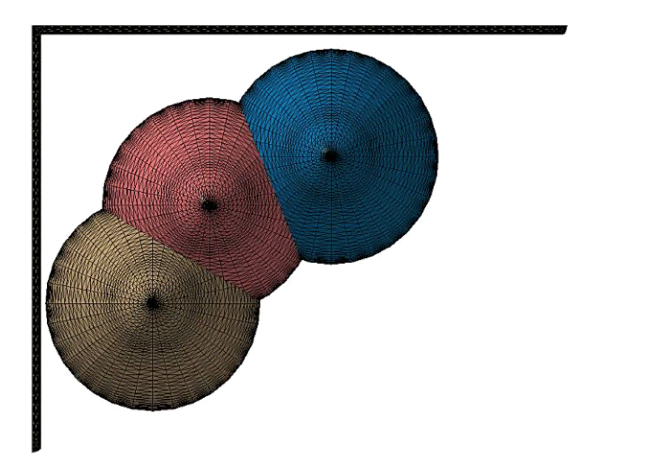
\includegraphics[width=0.28\textwidth]{reservoir_projection.png}}\\
 \subfigure[]{\label{fig:EIB_high}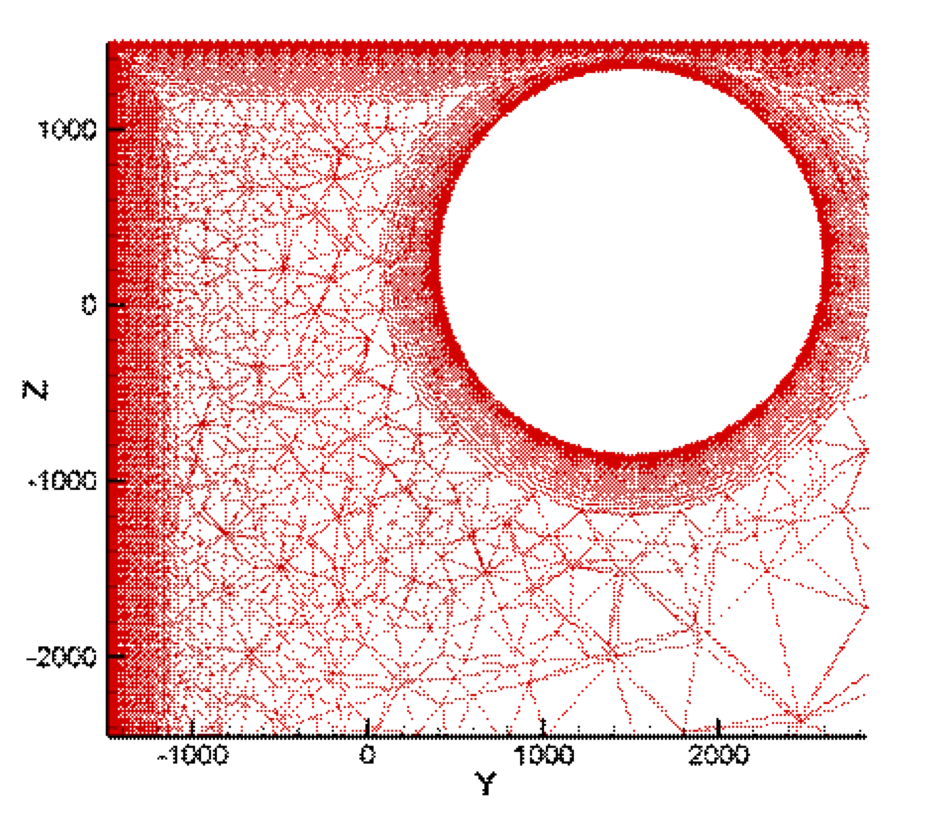
\includegraphics[width=0.25\textwidth]{reservoir_haut.png}}
 \subfigure[]{\label{fig:EIB_middle}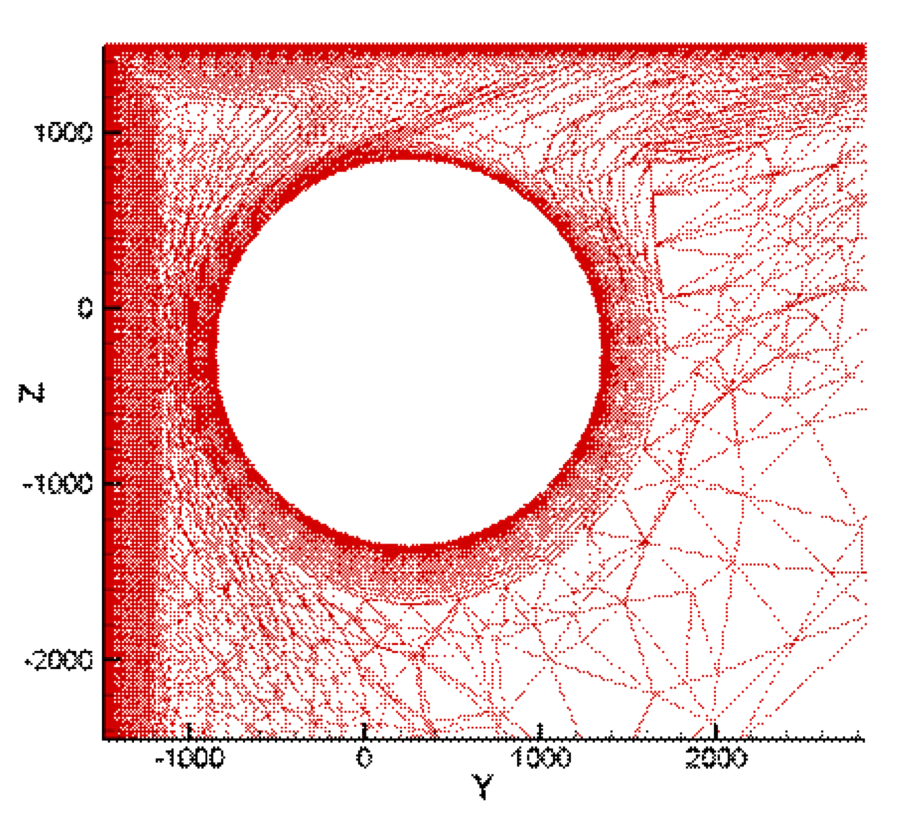
\includegraphics[width=0.246\textwidth]{reservoir_milieu.png}}
 \subfigure[]{\label{fig:EIB_bottom}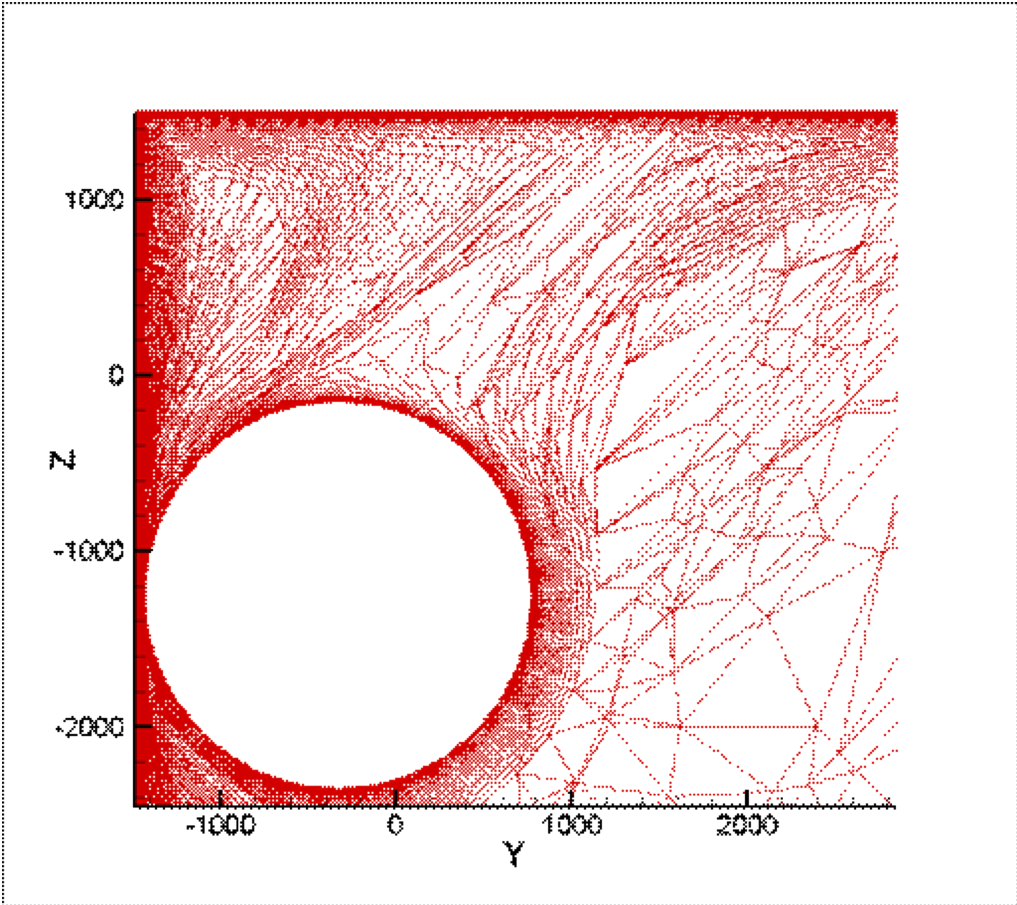
\includegraphics[width=0.249\textwidth]{reservoir_bas.png}}
 \caption{EIB fuel tank position optimization test case}
 \label{fig:reservoir}
\end{figure}

\subsection{Experimental Setup}
In the following experiments, we compare three versions of the FEM assembly step from the DEFMESH application:
the original domain decomposition version from Dassault Aviation called {\tt Ref}, the new Divide and Conquer version called {\tt D\&C}, and the coloring version called {\tt Coloring}.
The {\tt Ref} version uses MPI between the different blocks of the mesh and OpenMP to parallelize the sparse matrix-vector loop of the solver.
The {\tt D\&C} version uses the recursive partitioning of each block of the mesh.
In addition to MPI and OpenMP, this version exploits the task parallelism in the FEM assembly using Cilk.
The {\tt Coloring} version exploits OpenMP parallelism between all the elements of a same color in the FEM assembly.

For each of these versions, we consider the non-linear algorithm of the Laplacian and the Elastic operators of DEFMESH.
Both of them run in 50 linear steps.
The measures correspond to the average time of one iteration.
We measure the FEM assembly step, where the D\&C approach and the coloring have been applied.
We also measure the solver to estimate the impact of the D\&C data permutations on the rest of the code.
We ensure that the numerical results and the number of solver iterations needed to converge are stable in all versions.

We present the results both in terms of execution times and of parallel efficiency.
When the \emph{x} axis represents the number of cores, it corresponds to the number of MPI processes multiplied by the number of threads.
In the figures presenting execution time, the \emph{y} axis corresponds to elapsed CPU cycles for the FEM assembly and to elapsed time for the solver.
Concerning efficiency, the \emph{y} axis represents the parallel efficiency given by the following formula:
$E_{P} = \frac{T_{S}}{P*T_{P}}$, where $E_{P}$ is the efficiency on $P$ processor, $T_{S}$ the sequential time, and $T_{P}$ the time on $P$ processors.

For each figure, we use 1, 4, 8 and 12 MPI processes for {\tt Ref} and 1 MPI with 1, 2, 4, 6, 8 and 12 threads for {\tt Coloring} and {\tt D\&C}.
We also vary the number of METIS partitions and the number of Cilk tasks, but we did not observe significant changes in the results.
According to the Cilk documentations, a minimum of 10 tasks per core is appropriate.
Therefore we use 128 Cilk tasks, which is enough to fit in cache.
We cut MPI domains in 512 partitions to improve locality.

The application has been compiled with Intel composers 13.1.1 (icc and ifort) and Intel MPI 4.1.0 and Intel Cilk+ runtime.
The OpenMP affinity is set to scatter and Cilk threads are not pinned.
We perform these experiments on twelve cores grouped in two sockets of 6 cores Intel Xeon X5650 clocked at 2.67 GHz.
Each core has its own L1 (32KB) and L2 (256KB) caches and a shared L3 cache of 12MB. The main memory is divided in two NUMA nodes of 16GB.

\subsection{FEM Assembly results}
\begin{figure}[htp]
 \subfigure[Laplacian execution time]{\label{fig:asmCurvesA}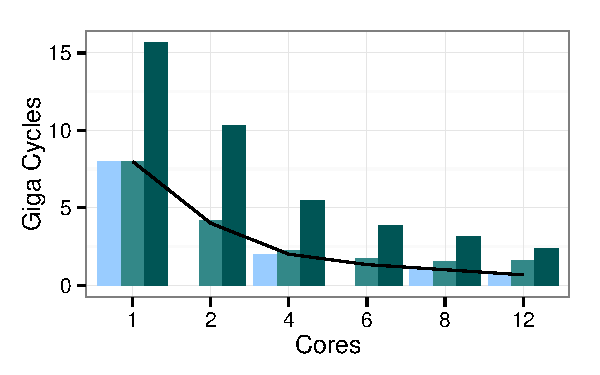
\includegraphics[width=0.43\textwidth]{graph_R/Laplacian_asm_time.pdf}}
 \subfigure[Laplacian parallel efficiency]{\label{fig:asmCurvesB}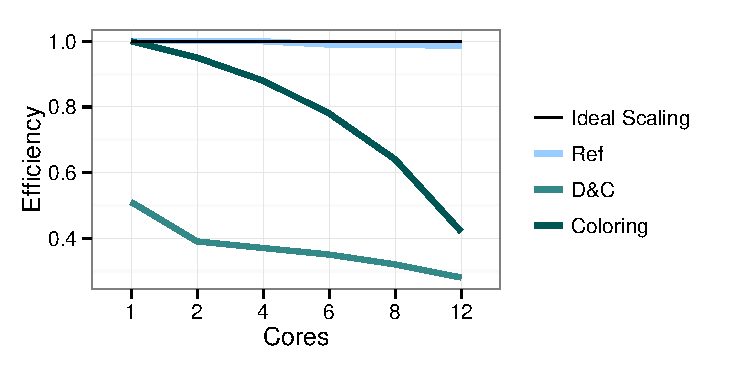
\includegraphics[width=0.55\textwidth]{graph_R/Laplacian_asm_efficiency.pdf}}
 \subfigure[Elasticity execution time]{\label{fig:asmCurvesC}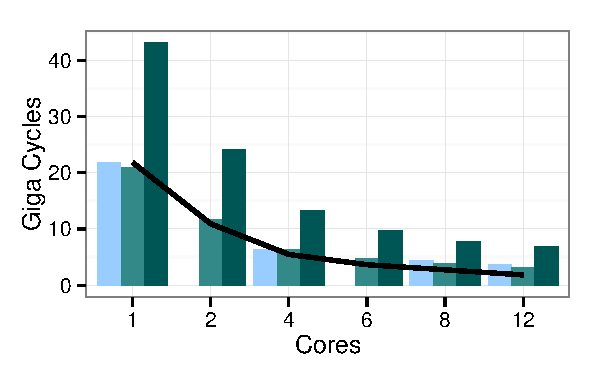
\includegraphics[width=0.43\textwidth]{graph_R/Elasticity_asm_time.pdf}}
 \subfigure[Elasticity parallel efficiency]{\label{fig:asmCurvesD}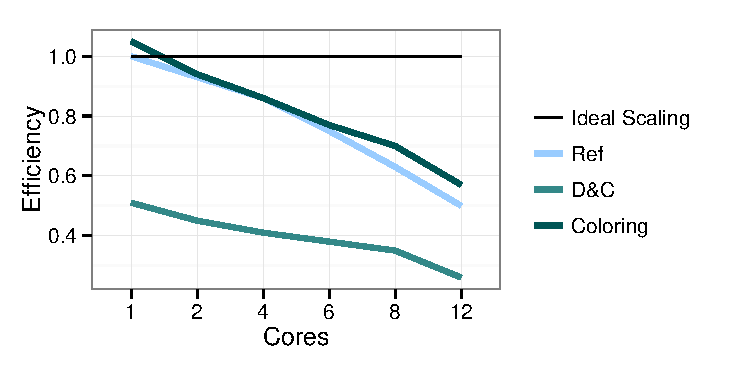
\includegraphics[width=0.55\textwidth]{graph_R/Elasticity_asm_efficiency.pdf}}
 \caption{FEM assembly time and efficiency measurement for the Laplacian and Elasticity version.}
 \label{fig:asmCurves}
\end{figure}

As we can see in Figure~\ref{fig:asmCurvesA} representing the Laplacian variant, the {\tt D\&C} version is close to the {\tt Ref} version, using MPI domain decomposition, but it starts to decrease after 6 cores.
This is due to the remaining sequential part of the D\&C code and the low intensity work in the Laplacian version.
Indeed, separator elements are not parallelized and can represent an important proportion of the computation.
According to the Amdahl's law, by increasing the number of cores, the proportion of the sequential part increases.
This is confirmed on Figure~\ref{fig:asmCurvesB} showing the parallel efficiency.

In the Elasticity variant, illustrated in Figures~\ref{fig:asmCurvesC} and~\ref{fig:asmCurvesD}, {\tt D\&C} becomes equivalent to {\tt Ref}.
Since the amount of work of the FEM assembly step is larger than in the Laplacian variant, the proportion of sequential computation, including the separators, is lower.
In this case the scalability improves.
Unlike the original version that makes irregular accesses to the cells of the matrix, the D\&C version works on matrix cells packed contiguously in small sub-matrix corresponding to the Cilk tasks.
For any problem size, with D\&C, we can increase the number of partitions so that the tasks working-set will always fit in cache.
When focusing on twelve cores, see Figure~\ref{fig:12CoresA}, all combinations of the {\tt D\&C} version are faster than {\tt Ref}.
In all variants, the {\tt Coloring} version is the slowest one.
This is probably due to a bad cache utilization as illustrated in Figure~\ref{fig:12CoresB}.

These first results are encouraging and we can reasonably expect to match the ideal scaling when the separators will be parallelized.

\begin{figure}[htp]
 \subfigure[$MPIxThreads (Version)$]{\label{fig:12CoresA}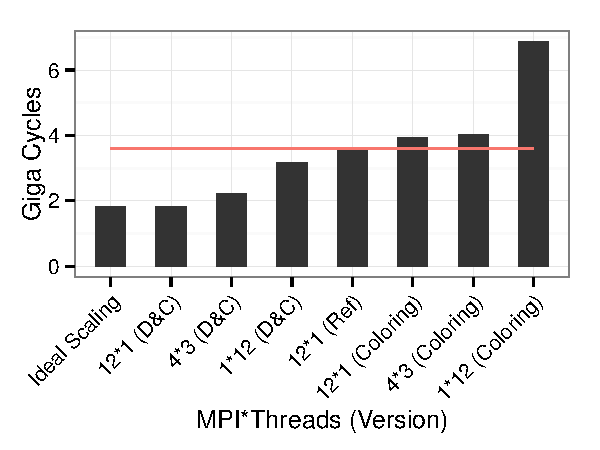
\includegraphics[width=0.4\textwidth]{graph_R/Elasticity_asm_time_12_cores.pdf}}
 \subfigure[$MPIxThreads (Version)$]{\label{fig:12CoresB}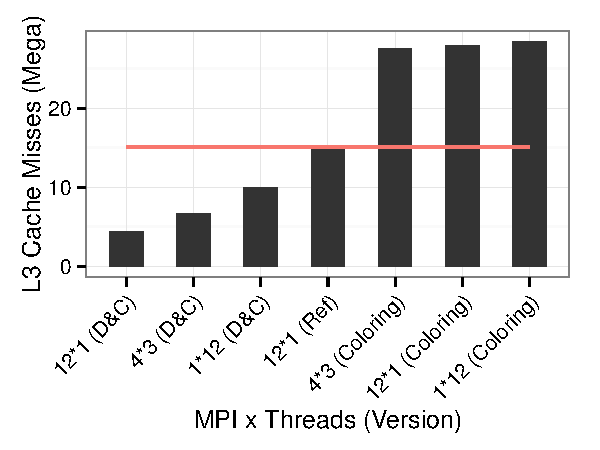
\includegraphics[width=0.4\textwidth]{graph_R/Elasticity_asm_L3TCM.pdf}}
 \caption{Comparison between all Elasticity versions on 12 cores. Execution time (a). L3 cache misses (b)}
 \label{fig:12Cores}
\end{figure}

\subsection{Solver}
\begin{figure}[htp]
 \subfigure[D\&C solver speed-up over Ref]{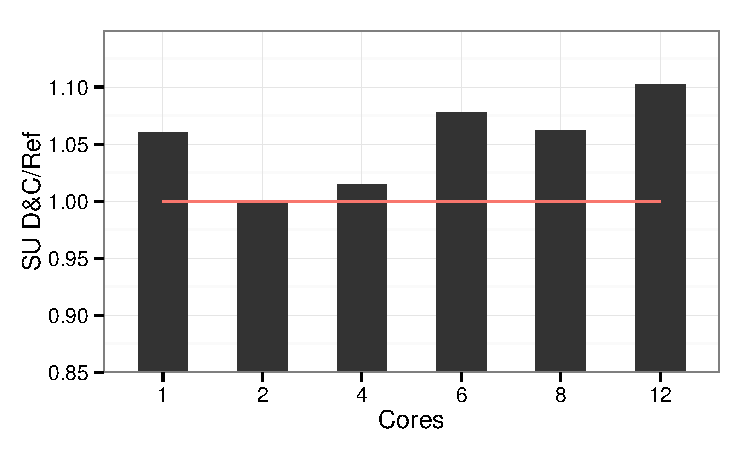
\includegraphics[width=0.43\textwidth]{graph_R/Laplacian_solver_time_SU.pdf}}
 \subfigure[Solver execution time]{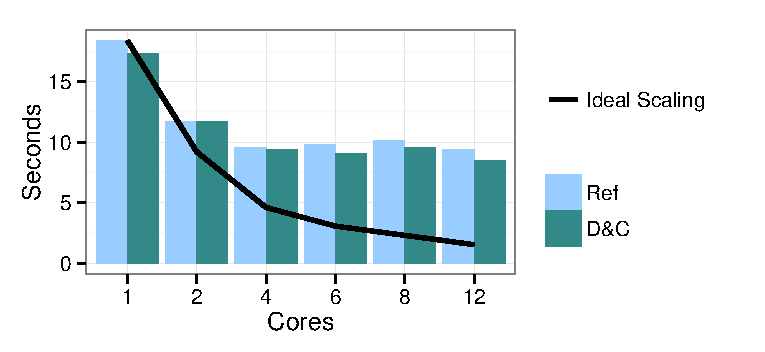
\includegraphics[width=0.55\textwidth]{graph_R/Laplacian_solver_time.pdf}}
 \caption{Solver execution time and speed-up using D\&C}
 \label{fig:solCurves}
\end{figure}

We did not modify the solver part.
However, we observe in Figure~\ref{fig:solCurves} an average 6\% speed-up for {\tt D\&C} compared to {\tt Ref}.
The maximum speed-up is 10,2\% on twelve cores.
This improvement is due to the better data locality enabled by the permutations explained in Section~\ref{sec:DCrec}.
To show the impact of locality, we randomly permute the data and observe a significant degradation of performance.
This result shows that the initial data already expose good locality.
Moreover, the L3 cache misses occurring in the solver are 23\% lower with {\tt D\&C} than with {\tt Ref}.

%---------------------------------------------------------------------------
%---------------------------------------------------------------------------
%---------------------------------------------------------------------------
%---------------------------------------------------------------------------

\section{Related Work}
\label{sec:rw}

TODO cite~\cite{dc_specfem} and some Marc's papers

Many choices are available to complete FEM assembly in parallel.
All methods have their advantages and their limitations, depending for instance on the target architecture or the mesh size.
Recent studies~\cite{cecka2011assembly,CPUGPUasm} investigate different ways to compute FEM assembly on CPUs and GPUs.

A first method, presented in~\cite{cecka2011assembly}, consists in creating parallelism between all the non-zero entries of the system of equations.
This method has a very fine grain thread parallelism and thus can be applied only to GPUs.
It stores, in parallel, the contributions from all elements in the global or local memory and then reduce in parallel these contributions to compute the non-zero values.
By arranging the data layout, this method can provide good performance on GPUs.
However, it suffers from bad load balancing since the number of neighboring elements used to compute non-zero values may vary.
Due to the fast growing number of local copies, the approach is limited to relatively small test cases.
Another variant consists in using one thread for the assembly of one non-zero value at a time.
However, this approach leads to redundant computations of element contributions.

A second method~\cite{cecka2011assembly} consists in assembling by mesh element.
One thread is responsible for the contribution of one element.
It can be applied to both GPUs and CPUs.
A coloring approach~\cite{CUDAfe,CPUfe} can be used to launch several threads in parallel on independent elements.
This way, each thread has a good load balance per color.
The load balancing between colors has no influence since they are serialized.
However, bad data locality can cause poor performance as explained is Section~\ref{sec:col}.

Divide and Conquer paradigm and recursion in general have already been explored extensively for parallel algorithm~\cite{div}.
M. Martone et al.~\cite{RSBasm} describe a matrix assembly approach for recursive sparse blocks (RSB) matrix on CPUs.
Despite this format can provide good results in solver algorithms~\cite{RSBsolver}, FEM assembly on RSB matrix is memory-bandwidth bound~\cite{RSBasm} according to authors results.
Dongarra et al.~\cite{Dongarra} evaluate an asynchronous task based parallelism approach for well-known factorization algorithms and compare it to traditional fork-join approach.
A recent investigation on hybrid programming integrating task based parallelism in MPI processes have been made~\cite{MPI_task}.
The experiments done on a 1024 nodes cluster result in significant speed-up on several micro-benchmarks and strong scaling applications compared to MPI domain decomposition.
However, recursive and D\&C approaches are rarely employed on sparse algebra and unstructured problems because of their irregularity.

%---------------------------------------------------------------------------
%---------------------------------------------------------------------------
%---------------------------------------------------------------------------
%---------------------------------------------------------------------------

\section{Conclusion and Future Work}
\label{sec:conc}
FEM assembly is the first step of many applications, such as seismic simulation, metal forming simulations, or crash test simulations.
Depending on the application, the FEM assembly can represent more than 80\% of the execution time.
In the Dassault Aviation DEFMESH application, the current D\&C implementation is already faster than the original  MPI domain decomposition version and overpasses in performance and scalability the state-of-the-art coloring approach.
Even without exploiting the thread level parallelism, the D\&C approach significantly improves the locality, the scalability, and the execution time.
The MPI domain decomposition version with D\&C has a perfect strong scaling for our experimental setup.

As a future work, we plan to parallelize the separator in the D\&C FEM assembly and experiment on a larger number of cores.
We strongly believe that D\&C will provide good performances on new manycores such as Xeon Phi.
Extension will focus on D\&C friendly data structure definition and apply D\&C on other parts of the FEM application. 
%We are also considering a hybrid approach using coloring inside each D\&C sub-domains in order to enable vectorization.

\subsubsection*{Acknowledgments} \scriptsize{
This work has been supported by the ITEA2 project H4H, the French Ministry for Economy,
Industry, and Employment, CEA, GENCI, Intel and UVSQ.  Any opinions,
findings, and conclusions or recommendations expressed in this
material are those of the author(s) and do not necessarily reflect the
views of the CEA, GENCI, Intel, Dassault Aviation or UVSQ.}

\bibliographystyle{unsrt}
\bibliography{dc_bib}

\end{document}